\chapter{Introduction}
\label{chap:intr}

\section{Basics}
\label{sec:basics}

Pole shifting theorem is one of the basic results of the theory of linear dynamical systems with linear feedback. It claims that in case of controllable systems one can achieve an arbitrary asymptotic behavior by a suitably chosen feedback. To understand this crucial theorem, we must first describe few basic concepts.

\subsection{Systems of First Order Differential Equations}

\begin{remark}
	Let $f(t)$ be a function of time $t\in\R^+$. We will denote its derivative with respect to $t$ by $$\dot{f}(t)=\frac{d}{dt}f(t)\ .$$
\end{remark}

\begin{definition}
	A \termdef{system of linear differential equations of order of one with constant coefficients} is a system 
	\begin{align*}
		\dot{x}_1(t)&=a_{1,1}x_1(t)+\ldots+a_{1,n}x_n(t) \\
		&\vdotswithin{=} \\
		\dot{x}_n(t)&=a_{n,1}x_1(t)+\ldots+a_{n,n}x_n(t)\ .
	\end{align*}
	The system can be written in a matrix form $$\dot{x}(t)=Ax(t)\ ,$$ where $x(t)=(x_1(t),\ldots,x_n(t))^T \in \C^n$ is a \termdef{state vector} (shortly \termdef{state}) of the system. The matrix $A\in \C^{n\times n}$, $A=(a_{i,j})$ is a \termdef{fundamental matrix} of the system. The \termdef{initial condition} of the system is the state $x(0)$.
\end{definition}

We will use the matrix form, as it is a very compact way of describing the system.

To express solution of this system in similarly compact way we will establish the notion of a matrix exponential.

\begin{definition}
	Let $X$ be a real or complex square matrix. The exponential of $X$, denoted by $e^X$, is the square matrix of the same type defined by the series $$e^{X}=\sum _{k=0}^{\infty}\frac{1}{k!}X^{k}\ ,$$
	where $X^0$ is defined to be the identity matrix $I$ of the same type as $X$.
\end{definition}

For this definition to make sense, we need to show that the series converges for any real or complex square matrix. Firstly, we will define what does it mean for a matrix series to converge. In this text, we will be using Frobenius norm to describe the notion of the convergence of a matrix series.

\begin{definition}
	\termdef{Frobenius norm} is a matrix norm, denoted by $\norm{\cdot}_F$, which for an arbitrary $n \times m$ matrix $A$ is defined as $$\norm{A}_F=\sqrt{\sum^n_{i=1}\sum^m_{j=1}\abs{a_{i,j}}^2}\ .$$
\end{definition}

\begin{remark}
	In what follows, $\K$ will denote a field of either real or complex numbers.
\end{remark}

\begin{lemma}
\label{lem:frobNormProperties}
	Then Frobenius norm satisfies following statements for any matrices $A$, $B$, $C\in \K^{n \times m}$, $D\in\K^{m\times o}$ and any scalar $\alpha \in \K$.
	\begin{enumerate}
		\item $\norm{A+B}_F\leq\norm{A}_F+\norm{B}_F\ ,$
		\item $\norm{\alpha A}_F=\abs{\alpha}\norm{A}_F\ ,$
		\item $\norm{A}_F\geq 0$ with equality occurring if and only if $A=O_{n \times m}\ ,$
		\item $\norm{CD}_F\leq\norm{C}_F\norm{D}_F\ .$
	\end{enumerate}
\end{lemma}

\begin{proof}
	First three points can be simply shown using the definition of the Frobenius form and properties of the absolute value. 

	The forth point follows from the Cauchy–Schwarz inequality 
	$$\norm{CD}^2_F=\sum^m_{i=1}\sum^o_{j=1}\norm{c_id_j}_2^2 \leq \sum^m_{i=1}\sum^o_{j=1}\norm{c_i}_2^2\norm{d_j}_2^2=\sum^m_{i=1}\norm{c_i}_2^2\sum^o_{j=1}\norm{d_j}_2^2=\norm{C}^2_F\norm{D}^2_F\ ,$$
	where $\norm*{\cdot}_2$ denotes the Euclidean norm, and $c_i,d_i$ denote the $i$-th column of the matrices $C$ and $D$ respectively.
\end{proof}

\begin{lemma}
\label{lem:elementAbsoluteSize}
	Absolute value of any element of a matrix is always less than or equal to the Frobenius norm of the matrix. In particular, for a matrix $A^k=(a_{i,j}^{(k)})_{n\times n}$, where $A\in\K^{n\times n}$, for every position $(i,j)$ it holds $\abs*{a_{i,j}^{(k)}}\leq\norm*{A^k}_F\leq\norm{A}^k_F$.
\end{lemma}

\begin{proof}
	Obviously, for an arbitrary element of the matrix $X=(x_{i,j})_{n\times m}$ we can write $$\abs*{x_{i,j}}\leq \sqrt{\sum^n_{i=1}\sum^m_{j=1}\abs*{x_{i,j}}^2}=\norm{X}_F\ .$$ It follows 
	$$\abs*{a_{i,j}^{(k)}}\leq\norm*{A^k}_F\leq\norm{A}^k_F\ ,$$
	where second inequality follows from Lemma \ref{lem:frobNormProperties}.4.
\end{proof}

\begin{cor}
	\label{cor:elementConvergence}
	Let us have $A^k=(a_{i,j}^{(k)})_{n\times n}$. Then the series $\sum^\infty_{k=0}\frac{b^k}{k!}a_{i,j}^{(k)}$ converges absolutely for any $b\in\K$.
\end{cor}

\begin{proof}
	By Lemma \ref{lem:elementAbsoluteSize}, for any $N\in\N$, we have
	$$\sum^N_{k=0}\abs{\frac{b^k}{k!}a_{i,j}^{(k)}}\leq\sum^N_{k=0}\frac{\abs{b}^k}{k!}\abs{a_{i,j}^{(k)}}\leq\sum^N_{k=0}\frac{\abs{b}^k}{k!}\norm{A}_F^{k}=\sum^N_{k=0}\frac{\norm{bA}_F^k}{k}$$
	Then 
	$$\sum^\infty_{k=0}\abs{\frac{b^k}{k!}a_{i,j}^{(k)}}=\lim_{N\to\infty}\sum^N_{k=0}\abs{\frac{b^k}{k!}a_{i,j}^{(k)}}\leq\lim_{N\to\infty}\sum^N_{k=0}\frac{\norm{bA}_F^k}{k}=\sum^\infty_{k=0}\frac{\norm{bA}_F^k}{k}=e^{\norm{bA}_F}$$
\end{proof}

\begin{definition}
	A matrix sequence $\{A_k\}_{k=0}^\infty$ of $n \times m$ matrices is said to \termdef{converge} to $n\times m$ matrix $A$, denoted by $A_k\longrightarrow A$, if $$\forall\varepsilon\in\R, \varepsilon>0\quad\exists n_0\in\N\quad\forall n\in\N,n\geq n_0:||A_n-A||_F<\varepsilon\ .$$
\end{definition}

\begin{lemma}
\label{lem:elementwiseConvergence}
	A matrix sequence $\{A_k=(a^{(k)}_{i,j})_{n\times m}\}_{k=0}^\infty$ converges to a matrix $A=(a_{i,j})_{n\times m}$ if and only if it converges elementwise, in other words $$\forall i\in\{1,\ldots,n\}\quad\forall j\in\{1,\ldots,m\} : a^{(k)}_{i,j}\xrightarrow{k\rightarrow\infty}a_{i,j}\ .$$
\end{lemma}

\begin{proof}
	Let $A_k \rightarrow A$. Then we can for any $\varepsilon>0$ find such $n_0$ that $\norm{A_n-A}_F<\varepsilon$ for every $n\geq n_0$. Using Lemma \ref{lem:elementAbsoluteSize} we can write $$\abs*{a^{(n)}_{i,j}-a_{i,j}}\leq \norm{A_n-A}_F<\varepsilon\ .$$ It follows that $\{A_k\}_{k=0}^\infty$ converges to $A$ elementwise.

	Conversely, let $\varepsilon$ be a positive real number. For every position $(i,j)$ we find such $n_{i,j}$ that $$\forall n\geq n_{i,j}:\abs*{a^{(n)}_{i,j}-a_{i,j}}<\frac{\varepsilon}{\sqrt{nm}}\ .$$ We put $N_0=\text{min}\{n_{i,j}\}$. Now $\forall n\in\N, n\geq N_0$ we have $$||A_n-A||_F=\sqrt{\sum^n_{i=1}\sum^m_{j=1}|a^{(n)}_{i,j}-a_{i,j}|^2}<\sqrt{nm\frac{\varepsilon^2}{nm}}=\varepsilon\ .$$
\end{proof}

\begin{claim}
\label{claim:matrixExpConv}
	The definition of the matrix exponential makes sense, that is, the matrix series \label{lem:point:expConv} $\sum _{k=0}^{\infty}\frac{1}{k!}X^{k}$ converges for any matrix $X$.
\end{claim}

\begin{proof}
	Let $X^k=(x_{i,j}^{(k)})_{n\times n}$. By Corollary \ref{cor:elementConvergence} every element of matrix $\sum^\infty_{k=0}\frac{1}{k!}X^k=\left(\sum^\infty_{k=0}\frac{1}{k!}x^{(k)}_{i,j}\right)_{n\times n}$ converges absolutely. Therefore the matrix series converges elementwise to some matrix $Y$ (we denote this matrix by $e^X$).
\end{proof}

\begin{lemma}
\label{lem:matrixSeriesFactoring}
	Let $\{A_k\}_{k=0}^\infty$ be a matrix sequence, where $A_k\in\K^{n\times m}$, $B\in\K^{r\times n}$ and $C\in\K^{m\times s}$. If $\sum^\infty_{k=0}A_k$ converges, then also $\sum^\infty_{k=0}BA_kC$ converges, and the following equality holds
	$$B\left(\sum^\infty_{k=0}A_k\right)C=\sum^\infty_{k=0}BA_kC\ .$$
\end{lemma}

\begin{proof}
	We know that for $N\in\N$ it is true
	$$\sum^N_{k=0}BA_kC=B\left(\sum^N_{k=0}A_k\right)C\ .$$
	We want to now show that the left hand side converges to $B\left(\sum^\infty_{k=0}A_k\right)C$. Let $\varepsilon_1\in\R^+$ be fixed. Since the series $\sum^\infty_{k=0}A^k$ converges, we can find $N_0$ such that for every $N\in\N,N\geq N_0$ it holds 
	$$\norm{\sum^\infty_{k=0}A_k-\sum^N_{l=0}A_l}<\varepsilon_1\ .$$
	Then 
	\begin{align*}
		\norm{B\left(\sum^\infty_{k=0}A_k\right)C-\sum^N_{l=0}BA_lC}_F&=
		\norm{B\left(\sum^\infty_{k=0}A_k\right)C-B\left(\sum^N_{l=0}A_l\right)C}_F=\\
		=\norm{B\left(\sum^\infty_{k=0}A_k-\sum^N_{l=0}A_l\right)C}_F&=
		\norm{B}_F\norm{\sum^\infty_{k=0}A_k-\sum^N_{l=0}A_l}_F\norm{C}_F
		<\norm{B}_F\norm{C}_F\varepsilon_1\ .
	\end{align*}
	That concludes the proof that $\sum^\infty_{k=0}BA_kC$ converges to $B\left(\sum^\infty_{k=0}A_k\right)C$.
\end{proof}

\begin{definition}
	Let us have a matrix function $X(t)\colon\R\rightarrow\K^{n\times m}$. Then the derivative of the function is $$\frac{d}{dt}X(t)=\left(\frac{d}{dt}x_{i,j}(t)\right)_{n\times m}=\Big(\dot{x}_{i,j}(t)\Big)_{n\times m}\ .$$
\end{definition}

\begin{lemma}
\label{lem:expprop}
	Let $A$, $B$ and $X$ be real or complex $n\times n$ matrices. Then 
	\begin{enumerate}
		\item If $AB = BA$, then $e^{A}B = Be^{A}$,
		\item If $R$ is invertible, then $e^{R^{-1}XR}=R^{-1}e^XR$,
		\item $\frac{d}{dt}e^{tX}=Xe^{tX}$, for $t \in \R$,
		\item If $AB = BA$, then $e^{A+B} = e^{A}e^B$.
	\end{enumerate}
\end{lemma}

\begin{proof}
	\begin{enumerate}
		\item
		Because of the convergence of the matrix exponential, we can use Lemma \ref{lem:matrixSeriesFactoring} and we get
		$$e^{A}B=\sum^\infty_{k=0}\frac{1}{k!}A^{k}B\stackrel{AB=BA}{=\joinrel=\joinrel=}\sum^\infty_{k=0}\frac{1}{k!}BA^{k}=B\sum^\infty_{k=0}\frac{1}{k!}A^{k}=Be^{A}\ .$$
		
		\item Following from Lemma \ref{lem:matrixSeriesFactoring}, we have 
		\begin{longeq}
			e^{R^{-1}XR}=\sum^\infty_{k=0}\frac{1}{k!}(R^{-1}XR)^{k}=\sum^\infty_{k=0}\frac{1}{k!}R^{-1}X^{k}R=R^{-1}\left(\sum^\infty_{k=0}\frac{1}{k!}X^{k}\right)R=R^{-1}e^{X}R\ . 
		\end{longeq}

		\item The elements of the matrix $e^{tX}=\sum^\infty_{k=0}\frac{t^k}{k!}X^{k}=(e_{i,j}(t))_{n\times n}$ are equal to
		$$e_{i,j}(t)=\sum^\infty_{k=0}\frac{t^k}{k!}a^{(k)}_{i,j}\ ,$$
		where $X^k=(a^{(k)}_{i,j})_{n\times n}$. By Corollary \ref{cor:elementConvergence} the series $\sum^\infty_{k=0}\frac{t^k}{k!}a^{(k)}_{i,j}$ is absolutely convergent for every $t\in\K$. We can now differentiate the individual elements (see \cite{Pick}, Věta 8.2.2.)
		$$\frac{d}{dt}e_{i,j}(t)=\frac{d}{dt}\sum^\infty_{k=0}\frac{t^k}{k!}a^{(k)}_{i,j}=\sum^\infty_{k=1}\frac{t^{k-1}}{(k-1)!}a^{(k)}_{i,j}=\sum^\infty_{k=0}\frac{t^{k}}{k!}a^{(k+1)}_{i,j}\ .$$ 
		Using Lemma \ref{lem:matrixSeriesFactoring} we get the desired result
		\begin{longeq}
			\frac{d}{dt}e^{tX}=\left(\frac{d}{dt}e_{i,j}(t)\right)_{n\times n}=\left(\sum^\infty_{k=0}\frac{t^{k}}{k!}a^{(k+1)}_{i,j}\right)_{n\times n}=\sum^\infty_{k=0}\frac{t^k}{k!}X^{k+1}=X\sum^\infty_{k=0}\frac{t^k}{k!}X^{k}=Xe^{tX}\ .
		\end{longeq}

		\item Let us denote elements of matrix $A^kB^l=(\alpha^{(k,l)}_{i,j})_{n\times n}$. Then
		\begin{align*}
			e^{A}e^{B}
			&=\sum^\infty_{k=0}\frac{1}{k!}A^{k}\cdot\sum^\infty_{l=0}\frac{1}{l!}B^{l}
			=\sum^\infty_{k=0}\left(\frac{1}{k!}A^{k}\sum^\infty_{l=0}\frac{1}{l!}B^{l}\right)
			=\sum^\infty_{k=0}\sum^\infty_{l=0}\frac{1}{k!l!}A^kB^l
			\\
			&=\left(\sum^\infty_{k=0}\sum^\infty_{l=0}\frac{1}{k!l!}\alpha^{(k,l)}_{i,j}\right)_{n\times n}
			=\left(\sum^\infty_{k=0}\sum^k_{l=0}\frac{1}{l!(k-l)!}\alpha^{(l,k-l)}\right)_{n\times n}
			\\
			&=\sum^\infty_{k=0}\sum^k_{l=0}\frac{1}{l!(k-l)!}A^{l}B^{k-l}
			=\sum^\infty_{k=0}\sum^k_{l=0}\binom{k}{l}\frac{1}{k!}A^{l}B^{k-l}
			\\
			&=\sum^\infty_{k=0}\frac{1}{k!}(A+B)^{k}
			=e^{A+B}\ .
		\end{align*}
		The second and the third equalities hold by Lemma \ref{lem:matrixSeriesFactoring}, and the penultimate equality holds by the assumption $AB=BA$. The crucial point is the fifth equality in which we reorder the elements of the series as depicted in Figure \ref{fig:reordering}. 
		\begin{figure}[hp]
			\centering
			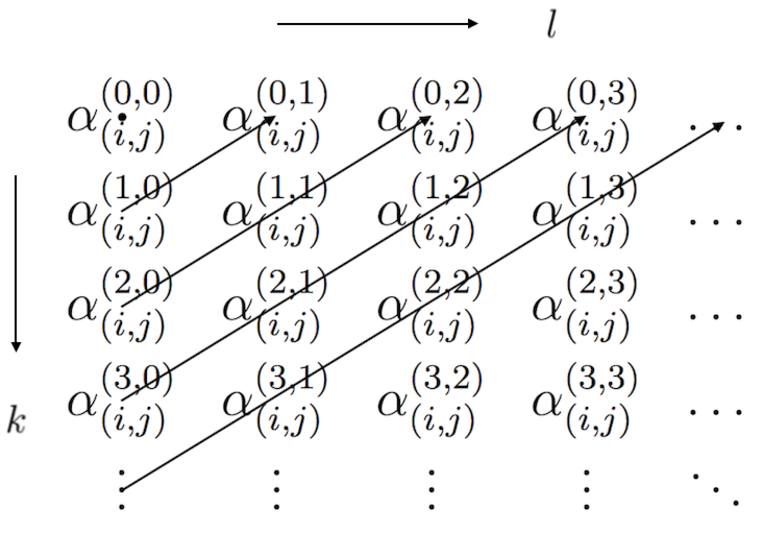
\includegraphics[width=70mm]{reordering_cropped.pdf}
			\captionsetup{justification=centering,margin=2cm}
			\captionof{figure}{}
			\label{fig:reordering}
		\end{figure}
		%\begingroup
		%\renewcommand*{\arraystretch}{1.5}
		%$$
		%\begin{matrix}
		%	\alpha^{(0,0)}_{(i,j)} & \alpha^{(0,1)}_{(i,j)} & \alpha^{(0,2)}_{(i,j)} & \alpha^{(0,3)}_{(i,j)} & \ldots \\
		%	\alpha^{(1,0)}_{(i,j)} & \alpha^{(1,1)}_{(i,j)} & \alpha^{(1,2)}_{(i,j)} & \alpha^{(1,3)}_{(i,j)} & \ldots \\
		%	\alpha^{(2,0)}_{(i,j)} & \alpha^{(2,1)}_{(i,j)} & \alpha^{(2,2)}_{(i,j)} & \alpha^{(2,3)}_{(i,j)} & \ldots \\
		%	\alpha^{(3,0)}_{(i,j)} & \alpha^{(3,1)}_{(i,j)} & \alpha^{(3,2)}_{(i,j)} & \alpha^{(3,3)}_{(i,j)} & \ldots \\
		%	\vdots & \vdots & \vdots & \vdots & \ddots
		%\end{matrix}
		%$$
		%\endgroup
		The equality holds as long as the original series is absolutely convergent. This follows from the inequality  
		$$\sum^N_{k=0}\sum^M_{l=0}\abs{\frac{1}{k!l!}\alpha^{(k,l)}_{i,j}}\leq\sum^N_{k=0}\frac{\norm{A}^k_F}{k!}\sum^M_{l=0}\frac{\norm{B}^l_F}{l!}=\left(\sum^N_{k=0}\frac{\norm{A}^k_F}{k!}\right)\cdot\left(\sum^M_{l=0}\frac{\norm{B}^l_F}{l!}\right)\ ,$$
		and the fact that the expression on the rightmost side is bounded by $e^{\norm{A}_F}e^{\norm{B}_F}$ for $M,N\rightarrow\infty$.
	\end{enumerate}
\end{proof}

\begin{lemma}
	\label{lem:matrixExpIdentity}
	For any $\alpha\in\K$ we have $e^{\alpha I}=e^{\alpha}I$.
\end{lemma}

\begin{proof}
	Follows straight from the definition of the matrix exponential.
\end{proof}

Now, using properties in Lemma \ref{lem:expprop}, we can see that $\dot{x}(t)=Ax(t)$ is solved by $x(t)=e^{tA}x(0)$. The solution is unique which follows from advanced calculus. Let us now discuss under what circumstances does the state $x(t)$ converge to $\nullvector$ for $t\rightarrow\infty$. 

Let $A$ be a real or complex matrix. Then there is a regular matrix $R\in \K^{n\times n}$ such that the matrix $$J=R^{-1}AR$$ is in the Jordan normal form. By substituting $x(t)=Ry(t)$, which is equivalent with changing the basis of our system, we get 
\begin{align*}
	R\dot{y}(t)&=ARy(t) \\
	\dot{y}(t)&=R^{-1}ARy(t) \\
	\dot{y}(t)&=Jy(t)
\end{align*}
and therefore the unique solution is $$y(t)=e^{tJ}y(0)\ ,$$ where $y(0)=R^{-1}x(0)$. It is sufficient to show that $y(t)$ converges to \nullvector, because since $R$ is an invertible matrix,  $x(t)$ converges to $\nullvector$ if and only if $y(t)$ converges to $\nullvector$.

We know that every Jordan block $J_{\lambda,n}$ in the matrix $J$ can be decomposed as $J_{\lambda,n}=\lambda I_n+N_n$, $n \in\N$ where $N_n$ is $n \times n$ nilpotent matrix satisfying $n_{i,j}=\delta_{i,j-1}$. For example, in case of $n=4$ we have
\begin{equation*}
	N_4=
	\begin{pmatrix}
		0 & 1 & 0 & 0 \\
		0 & 0 & 1 & 0 \\
		0 & 0 & 0 & 1 \\
		0 & 0 & 0 & 0 
	\end{pmatrix},
	(N_4)^2=
	\begin{pmatrix}
		0 & 0 & 1 & 0 \\
		0 & 0 & 0 & 1 \\
		0 & 0 & 0 & 0 \\
		0 & 0 & 0 & 0 
	\end{pmatrix},
	(N_4)^3=
	\begin{pmatrix}
		0 & 0 & 0 & 1 \\
		0 & 0 & 0 & 0 \\
		0 & 0 & 0 & 0 \\
		0 & 0 & 0 & 0 
	\end{pmatrix}
	.
\end{equation*}
It is also true that $(N_n)^k_{i,j}=\delta_{i,j-k}$ and $(N_n)^n=O_{n \times n}$, since every right multiplication by matrix $N$ shifts the multiplied matrix's columns to the right by one column, that is, it maps matrix $(v_1,\ldots,v_n)$ onto $(\nullvector,v_1,\ldots,v_{n-1})$. 

By using Lemma \ref{lem:expprop}, we now for each Jordan block $J_{\lambda,n}$ have
$$e^{tJ_{\lambda,n}}=e^{t(\lambda I + N)}=e^{t\lambda I}e^{tN}=e^{\lambda t}e^{tN}\ .$$
Let $\lambda = a+ib$ where $a$,$b \in \R$. Then we have
$$e^{tJ_{\lambda,n}}=e^{at}e^{ibt}e^{tN}\ .$$
We know that $|e^{ibt}|=1$ and that
$$e^{tN}=\sum^\infty_{k=0}\frac{t^k}{k!}N^k=\sum^{n-1}_{k=0}\frac{t^k}{k!}N^k$$
since $(N_n)^n=O_{n \times n}$. Therefore, we can see that every element of matrix $e^{tN}$ is a polynomial in $t$ of degree less than $n$. It follows that $e^{tJ_{\lambda,n}}$ approaches $O_{n \times n}$ in infinity if
$$\lim_{t\to\infty}e^{at}t^{n-1}=0\ .$$
This holds for any $n\in\N$ as long as $a<0$. 

Because any block diagonal matrix to the power of any natural number preserves its block form, we can write
\begin{equation*}
	J=
	\begin{pmatrix}
		J_{\lambda_1,n_1} & 0 & \cdots & 0 \\
		0 & J_{\lambda_2,n_2} & \cdots & 0 \\
		\vdots & \vdots & \ddots & \vdots \\
		0 & 0 & \cdots & J_{\lambda_r,n_r}
	\end{pmatrix},
	\quad 
	e^J=
	\begin{pmatrix}
		e^{J_{\lambda_1,n_1}} & 0 & \cdots & 0 \\
		0 & e^{J_{\lambda_2,n_2}} & \cdots & 0 \\
		\vdots & \vdots & \ddots & \vdots \\
		0 & 0 & \cdots & e^{J_{\lambda_r,n_r}}
	\end{pmatrix}
	,
\end{equation*}
where zeroes in the matrices represent zero matrices of appropriate sizes. Therefore, since $y(0)$ is a constant vector, we see that $y(t)=e^{tJ}y(0)$ converges to $\nullvector$ if (and only if, because of the uniqueness of the solution) all the eigenvalues $\lambda_i$ of the matrix $A$ have negative real parts. As the last step, we calculate $x(t)=Ry(t)$ and $x(0)=Ry(0)$. We formulate this result into a theorem.

\begin{theorem}
	The system $\dot{x}=Ax(t)$ is stable if and only if all eigenvalues of the matrix $A$ have negative real parts.
\end{theorem}

\begin{example}
	Consider higher order differential equation $$x^{(n)}(t)+a_1x^{(n-1)}(t)+\ldots+a_{n-1}x'(t)+a_nx(t)=0\ ,$$ where $x(t)\colon\C\rightarrow\C$. This equation can be solved as a system of linear differential equations of first order $\dot{z}(t)=Az(t)$ by choosing fundamental matrix $A$ and state vector $z(t)$ as follows
	\begin{equation*}
		A=
		\begin{pmatrix}
			0 & 1 & 0 & \cdots & 0 \\
			0 & 0 & 1 & \cdots & 0 \\
			\vdots & \vdots & \vdots & \ddots & \vdots \\
			0 & 0 & 0 & \cdots & 1 \\
			-a_n & -a_{n-1} & -a_{n-2} & \cdots & -a_1
		\end{pmatrix}
		, z(t)=
		\begin{pmatrix}
			x(t) \\
			x'(t) \\
			\vdots \\
			x^{(n-1)}(t)
		\end{pmatrix}.
	\end{equation*}
\end{example}

\subsection{Linear System With Control}

\begin{definition}
	A \termdef{continuous dynamical linear system with control u} is a system of linear differential equations of first order with constant coefficients in the form $$\dot{x}(t)=Ax(t)+Bu(t)\ ,$$ where $x(t)\in\K^n$ is a \termdef{state vector} (shortly \termdef{state}) of the system, $A\in\K^{n\times n}$ is a \termdef{fundamental matrix} of the system, $B\in\K^{n\times m}$ is a \termdef{control matrix} of the system and $u(t)\in\K^m$ is a \termdef{control vector} of the system. The \termdef{initial condition} of the system is the state $x(0)$.

	We will call this system shortly $(A,B)$ system.
\end{definition}

In a general case, this is called an \termdef{open-loop control} system because the control is not dependent on previous state of the system.

TODO

We can imagine this system as follows. The first part of the right side, $Ax(t)$, of the equation $\dot{x}(t)=Ax(t)+Bu(t)$ can be thought of as the model of machine or event that we want to control and the second part, $Bu(t)$, as our control mechanism. The $B$ matrix is our ``control board'' and the control vector $u(t)$ is us deciding, which levers and buttons we want to push. 

Of course, if we want this system to be self-regulating, we cannot input our own values into $u(t)$, and therefore it has to be calculated from the current state of our system.

END TODO

\begin{definition}
	Let us have linear differential system with control $u(t)$ defined as
	$$u(t)=Fx(t)\ ,$$
	where $F\in\C^{m\times n}$ is a \termdef{feedback matrix}. This system is then called a \termdef{closed-loop control} system or a \termdef{linear feedback control} system.
\end{definition}

Typically, we require a feedback control system to stabilize itself back into its stable state after some disturbances. 

\begin{definition}
	We say that the system $(A,B)$ is \termdef{stable}, if it converges to the null vector.
\end{definition}

The feedback control system can be expressed as a first order linear differential system $$\dot{x}(t)=Ax(t)+BFx(t)=(A+BF)x(t)\ .$$ As discussed in the first section, we now know that the system converges to $\nullvector$ if all of the eigenvalues of matrix $A+BF$ have negative real parts. 

Therefore, the system can stabilize itself if we find such matrix $F \in \C^{n \times n}$ that all the eigenvalues of the matrix $A+BF$ have negative real parts. This requirement can be expressed through characteristic polynomial of the matrix $A+BF$, since roots of the characteristic polynomial of a matrix are precisely the eigenvalues of the matrix.

\begin{definition}
	Let $A$ be a $n\times n$ matrix. Then the \termdef{characteristic polynomial} of A, denoted by $\chi_A$, is defined as $$\chi_A(s)=\textnormal{det}(sI_n-A)\ .$$
\end{definition}

Through our observations we got to a conclusion, that we need to find a feedback matrix $F$ such that the characteristic polynomial of the matrix $A+BF$ is $$\chi_{A+BF}=(x-\lambda_1)(x-\lambda_2)\cdots(x-\lambda_n)\ ,$$ where all its roots $\lambda_1,\lambda_2,\ldots,\lambda_n \in \C$ have negative real parts. This leads to an important definition.

\begin{definition}
    Let $\K$ be a field and let $A \in \K^{n \times n}$, $B \in \K^{n \times m}$, $n,m \in \N$. We say that polynomial $\chi$ is \termdef{assignable} for the pair $(A,B)$ if there exists such matrix $F\in\K^{m \times n}$ that $$\chi_{A+BF}=\chi\ .$$
\end{definition}

The pole shifting theorem states, that if $A$ and $B$ are ``sensible'' in a sense that we will discuss in the next section, then an arbitrary monic polynomial $\chi$ of degree $n$ can be assigned to the pair $(A,B)$. It also claims that it is immaterial over what field $A$ and $B$ are.

\section{Controllable pairs}

In this section we will establish the notion of controllability. We will first explain this concept for \textit{discrete-time systems} and then we will show that the requirement for controllability of \textit{continuous-time systems} is the same as the one for \textit{discrete-time systems}.

\subsection{Discrete-time systems}

Let us have a continuous dynamical system $\dot{x}(t)=A_1x(t)$, where $A_1$ is a real or complex square matrix. We \textit{discretize} the time, that is, instead of using continuous real time values of $x(t)$ and $\dot{x}(t)$, we are interested in these values only at discrete \textit{sampling times} $0,\delta,2\delta,\ldots,k\delta,\ldots$ where $\delta\in\R^+$. We will denote the states at each sampling time as follows
$$x_k=x(k\delta)\ ,k\in\N_0\ .$$
The solution of this system is precisely $x(t)=e^{tA_1}x(0)$, as discussed in previous sections. For some $k\in\N$ we get $x_k=x(k\delta)=e^{k\delta A_1}x(0)$ and $x_{k+1}=e^{(k+1)\delta A_1}x(0)=e^{\delta A_1 +k\delta A_1}x(0)$ which by Lemma \ref{lem:expprop}.5 equals $x_{k+1}=e^{\delta A_1 +k\delta A_1}x(0)=e^{\delta A_1}e^{k\delta A_1}x(0)=e^{\delta A_1}x_k$.

Using Lemma \ref{lem:expprop} we obtain 
\begin{align*}
	x_{k+1}
	&=e^{(k+1)\delta A_1}x(0) \\
	&=e^{\delta A_1 +k\delta A_1}x(0) \\
	&=e^{\delta A_1}e^{k\delta A_1}x(0) \\
	&=e^{\delta A_1}x_k \\
	&=Ax_k
\end{align*}
by choosing $A=e^{\delta A_1}$. We see that we can calculate the next value of $x$ from its previous value. We will now define this system. The definition holds for any field $\K$.

\begin{definition}
	A \termdef{discrete dynamical linear system} is a system of equations
	$$x_{k+1}=Ax_k,\ k\in\N_0\ ,$$
	where $x_k\in \K^n$ is a \termdef{state vector} (shortly \termdef{state}) of the system, the matrix $A\in \K^{n\times n}$ is a \termdef{fundamental matrix} of the system. The \termdef{initial condition} of the system is the state $x(0)$.
\end{definition}

\begin{definition}
	A \termdef{discrete dynamical linear system with control u} is a system of equations
	$$x_{k+1}=Ax_k+Bu_k,\ k\in\N_0\ ,$$
	where $x_k\in\K^n$ is a \termdef{state vector} (shortly \termdef{state}) of the system, $A\in\K^{n\times n}$ is a fundamental matrix, $B\in\K^{n\times m}$ is a control matrix, $u_k\in\K^m$ is a control vector. The \termdef{initial condition} of the system is the state $x_0$.

	We will call this system \termdef{discrete $(A,B)$} system.
\end{definition}

\begin{definition}
	We say that a state $x$ can be \termdef{reached} in time $k\in\N_0$ if there exists such a sequence of control vectors $u_0,u_1,\ldots,u_k$ that for starting condition $x_0=\nullvector$ we get $x=x_k$, after $k$ iterations of $x_{l+1}=Ax_l+Bx_l$, where $l\in\{0,1,\ldots,k-1\}$.
\end{definition}

States that we can reach in set number of iterations in a open-loop control discrete-time systems can be derived as follows. From state $x_k$ and control vector $u_k$ is the next state $x_{k+1}$ computed by equation
$$x_{k+1}=Ax_k+Bu_k$$
The starting condition is $x_0=\textbf{o}$ and we can choose an arbitrary $u_k$. Then, for $k=0$ we have $$x_1=Ax_0+Bu_0=Bu_0 \in \text{Im}B.$$ For $k=1$ we get
$$x_2=Ax_1+Bu_1=ABu_0+Bu_1\in\text(AB|B)$$
It is clear, that
$$x_k\in\text{Im}(A^{k-1}B|\cdots|AB|B)$$
We can observe that $\text{Im}(B|AB|\cdots|A^kB) \subseteq \text{Im}(B|AB|\cdots|A^{k+1}B)$. By Cayley-Hamilton theorem we know that $\chi_A(A)=O_{n\times n}$. That means that $A^n$ can be expressed as linear combination of matrices $\{I,A,\ldots,A^{n-1}\}$ or equivalently that $A^nB$ can be expressed as linear combination of matrices $\{B,AB,\ldots,A^{n-1}B\}$. We now see that $\text{Im}(B|AB|\cdots|A^kB) \supseteq \text{Im}(B|AB|\cdots|A^{k+1}B)$ holds. It follows
\begin{equation}
\label{eq:cayleHamilReachable}
	\text{Im}(B|AB|\cdots|A^{n-1}B)=\text{Im}(B|AB|\cdots|A^{n-1}B|A^nB)
\end{equation}
Therefore, all the states we could ever reach are already in space
$$\text{Im}(B|AB|\cdots|A^{n-1}B)$$

\begin{definition}
	Let $\K$ be a field and let $A \in \K^{n \times n}$, $B \in \K^{n \times m}$, $n,m \in \N$. We define \termdef{reachable space} $\mathcal{R}(A,B)$ of the pair $(A,B)$ as $\text{Im}(B|AB|\cdots|A^{n-1}B)$.
\end{definition}

We have seen that by left multiplying $\mathcal{R}(A,B)$ by $A$, we get the same subspace. This leads to an important property of some subspaces.

\begin{definition}
	Let $V$ be a vector space, $W$ be its subspace and $f$ be a mapping from $V$ to $V$. We call $W$ an \termdef{invariant subspace} of $f$ if $f(W)\subseteq W$.

	We also say that $W$ is \termdef{$f$-invariant}. When $f=f_A$ for some matrix $A$, we also shortly say that W is \termdef{$A$-invariant}.
\end{definition}

\begin{remark}
	\label{rem:reachinv}
	$\mathcal{R}(A,B)$ is a $A$-invariant subspace.
\end{remark} 

The maximum dimension of $\mathcal{R}(A,B)$ is, of course, $n$. This leads us to important property of pair $(A,B)$, where we want to be able to get the system into any state in state space by controlling it with our control vector $u(t)$, i.e., choosing appropriate $u(t)$. Therefore, we desire that $\mathcal{R}(A,B)=\K^n$. The equivalent condition is $\text{dim}\mathcal{R}(A,B)=n$.

\begin{definition}
	Let $\K$ be a field and let $A \in \K^{n \times n}$, $B \in \K^{n \times m}$, $n,m \in \N$. The pair $(A,B)$ is \termdef{controllable} if $\textnormal{dim}\mathcal{R}(A,B)=n$.
\end{definition}

\subsection{Continuous-time systems}

\begin{remark}
	In this section we assume, that $\K$ is a field of either real or complex numbers and that $A\in\K^{n\times n}$, $B\in\K^{n\times m}$.
\end{remark}

We will now show that the condition for controllability of \textit{discrete-time systems} also characterizes controllable \textit{continuous-time systems}. For this we have to express solution of such system using matrices $A^iB$ for $i\in \N_0$. 

We utilize matrix exponential in solving system of inhomogeneous linear system $\dot{x}(t)=Ax(t)+Bu(t)$. By left multiplying it by $e^{-tA}$ we get
\begin{align*}
	e^{-tA}\dot{x}(t)-e^{-tA}Ax(t) &=e^{-tA}Bu(t) \\
	\frac{d}{dt} (e^{-tA}x(t)) &=e^{-tA}Bu(t) 
\end{align*}
Note, we used $-AA=A(-A)\Rightarrow e^{-tA}A=Ae^{-tA}$ from Lemma \ref{lem:expprop}. After integrating both sides with respect to $t$ on interval $(t_0,t_1)$ we have 
\begin{align*}
	[e^{-tA}x(t)]^{t_1}_{t_0}&=\int^{t_1}_{t_0}e^{-tA}Bu(t)dt \\
	e^{-t_1A}x(t_1)-e^{-t_0A}x(t_0)&=\int^{t_1}_{t_0}e^{-tA}Bu(t)dt \\
	x(t_1)&=e^{(t_1-t_0)A}x(t_0)+\int^{t_1}_{t_0}e^{(t_1-t)A}Bu(t)dt
\end{align*}

Now it is clear that in system where $x(0)=\nullvector$ can every state in time $t\in \R^+$ be expressed as $$x(t)=\int^t_0 e^{(t-s)A}Bu(s)ds$$

\begin{definition}
	We say that a state $x\in\K^n$ can be \termdef{reached in the time $t$}, if there exists a control $u(x)\colon[0,t]\rightarrow\K^m$ such that
	$$x=\int^t_0 e^{(t-s)A}Bu(s)ds\ .$$

	The set of all states that can be reached in the time $t$ is denoted by $\mathcal{R}^t$. The set $\mathcal{R}=\cup_{t\in\R^+}\mathcal{R}^t$ of all states that can be reached, is called a \termdef{reachable space}.
\end{definition}

\begin{definition}
	A $n$-dimensional continuous-time linear system is \termdef{controllable}, if $\mathcal{R}=\K^n$.
\end{definition}

\begin{theorem}
	The $n$-dimensional continuous-time linear system is controllable if and only if $\text{dim}\mathcal{R}(A,B)=n$.
\end{theorem}

\begin{proof}
	From discussion above we have 
	$$
		x(t)=\int^t_0e^{(t-s)A}Bu(s)ds
		=\int^t_0\sum^\infty_{k=0}\frac{(t-s)^k}{k!}A^kBu(s)ds
	$$
	The $n$-dimensional vector $w^{(k)}(s)=A^kBu(s)$ has elements $$w^{(k)}_i(s)=\sum^m_{j=1}\alpha^{(k)}_{i,j}u_j(s)$$ where $\alpha^{(k)}_{i,j}$ is the element of the matrix $A^kB$ on the position $(i,j)$. Therefore, the elements of $x(t)$ are
	$$
		x_i(t)
		=\int^t_0\sum^\infty_{k=0}\frac{(t-s)^k}{k!}w^{(k)}_ids
		=\int^t_0\sum^\infty_{k=0}\sum^m_{j=1}\frac{(t-s)^k}{k!}\alpha^{(k)}_{i,j}u_j(s)ds
	$$
	
	Now, in order to be able to modify this expression, we will prove that the series $\sum^\infty_{k=0}\frac{(t-s)^k}{k!}\alpha^{(k)}_{i,j}u_j(s)$ is convergent for every position $(i, j)$. This follows from
	\begin{longeq}
		\abs{\sum^\infty_{k=0}\frac{(t-s)^k}{k!}\alpha_{i,j}^{(k)}u_j(s)}\leq \sum^\infty_{k=0}\frac{\abs{t-s}^k}{k!}\abs*{\alpha_{i,j}^{(k)}}\abs*{u_j(s)}\leq\sum^\infty_{k=0}\frac{\norm{(t-s)A}_F^k}{k!}\norm{B}_F\abs*{u_j(s)}\leq\abs*{u_j(s)}\norm{B}_Fe^{\norm{(t-s)A}}\ ,
	\end{longeq}
	where the second inequality holds by Corollary \ref{cor:elementConvergence}, and the third inequality by the fact that we can factor constants $\norm{B}_F$ and $u_j(s)$ out of convergent number series $e^{\norm{(t-s)A}}$. Because of the absolute convergence, we can now swap the integral and the series:
	\begin{align*}
		x_i(t)
		&=\int^t_0\sum^\infty_{k=0}\sum^m_{j=1}\frac{(t-s)^k}{k!}\alpha^{(k)}_{i,j}u_j(s)ds
		=\int^t_0\sum^m_{j=1}\sum^\infty_{k=0}\frac{(t-s)^k}{k!}\alpha^{(k)}_{i,j}u_j(s)ds
		\\
		&=\sum^m_{j=1}\int^t_0\sum^\infty_{k=0}\frac{(t-s)^k}{k!}\alpha^{(k)}_{i,j}u_j(s)ds
		=\sum^m_{j=1}\sum^\infty_{k=0}\int^t_0\frac{(t-s)^k}{k!}\alpha^{(k)}_{i,j}u_j(s)ds
		\\
		&=\sum^m_{j=1}\sum^\infty_{k=0}\alpha^{(k)}_{i,j}\int^t_0\frac{(t-s)^k}{k!}u_j(s)ds
		=\sum^\infty_{k=0}\sum^m_{j=1}\alpha^{(k)}_{i,j}\int^t_0\frac{(t-s)^k}{k!}u_j(s)ds
		\\
		&=\sum^\infty_{k=0}\sum^m_{j=1}\alpha^{(k)}_{i,j}v^{(k)}_i(t)\ ,
	\end{align*}
	where $v^{(k)}(t)=\int^t_0\frac{(t-s)^k}{k!}u(s)ds$ is a vector of length $m$. Therefore, we have 
	$$x(t)=\sum^\infty_{k=0}A^kBv_k(t)=\sum^\infty_{k=0}A^kB\int^t_0\frac{(t-s)^k}{k!}u(s)ds$$
	Now it its clear that $$x(t) \in \text{Im}(B|AB|\ldots|A^kB|\ldots)=\text{Im}(B|AB|\ldots|A^{n-1}B)=\mathcal{R}(A,B)$$ 
	The first equality follows from the equality (\ref{eq:cayleHamilReachable}).
	
	If the system is controllable then $x(t)$ can be equal to any of the vectors of an arbitrary basis of $\K^n$. Therefore, we know that $n$ linearly independent vectors belong into $\mathcal{R}(A,B)$, and naturally it follows $\text{dim}\mathcal{R}(A,B)=n$.

	Conversely, if dimension of reachable space is equal to $n$ we then have $x(t)\in\mathcal{R}(A,B)=\C^n$, therefore the system is controllable.
\end{proof}

\subsection{Decomposition theorem}

\begin{lemma}
	\label{lem:invsubspc}
	Let $W$ be an invariant subspace of linear mapping $f\colon V \rightarrow V$. Then there exists a basis $C$ of $V$ such that 
	\begin{equation*}
		[f]^C_C=
		\begin{pmatrix}
			F_1 & F_2 \\
			0   & F_3 
		\end{pmatrix}
	\end{equation*}
	where $F_1$ is $r\times r$, $r=\text{dim}W$.
\end{lemma}

\begin{proof}
	Let $(w_1,\ldots,w_r)$ be an arbitrary basis of subspace $W$. We complete this sequence into basis $C$ of $V$ with vectors $v_1,\ldots,v_{n-r}$ where $n=\text{dim}V$, thus $C=(w_1,\ldots,w_r,v_1,\ldots,v_{n-r})$. We know that $$[f]^C_C=([f(w_1)]_C,\ldots,[f(w_r)]_C,[f(v_1)]_C,\ldots,[f(v_{n-r})]_C)$$ Since $W$ is an $A$-invariant subspace, it holds that $f(w_i)\in W$ and therefore, because of our choice of the basis $C$, the matrix $[f]^C_C$ is of the desired form.
\end{proof}

If $(A,B)$ is not controllable, then there exists subspace of our state space that is not affected by our input. This can be shown using following theorem.

\begin{theorem}
	\label{theorem:decomp}
	Let $(A,B)$ represent a dynamical system and let $\text{dim}\mathcal{R}(A,B)=r\leq n$. Then there exists invertible $n\times n$ matrix $T$ over $\K$ such that the matrices $\widetilde{A}:=T^{-1}AT$ and $\widetilde{B}:=T^{-1}B$ have the block structure 
	\begin{equation}
		\label{eq:decomp}
		\widetilde{A}=
		\begin{pmatrix}
			A_1 & A_2 \\
			0   & A_3 
		\end{pmatrix}
		\qquad
		\widetilde{B}=
		\begin{pmatrix}
			B_1  \\
			0
		\end{pmatrix}
	\end{equation}
	where $A_1$ is $r \times r$ and $B_1$ is $r \times m$.
\end{theorem}

\begin{proof}
	We know that $\mathcal{R}(A,B)$ is an $A$-invariant subspace (Remark \ref{rem:reachinv}). Using Lemma \ref{lem:invsubspc} on the matrix mapping $f_A$ we get a basis $C$ for which it holds that 
	$$[f_A]^C_C=[\text{id}]^K_C[f_A]^K_K[\text{id}]^C_K=[\text{id}]^K_CA[\text{id}]^C_K$$ 
	is in a block triangular form. By putting $T=[\text{id}]^C_K=C$ we get that $\widetilde{A}=[f_A]^C_C$ is now in the desired form.

	Consider now matrix mapping $f_B$. We have $$\widetilde{B}=TB=[\text{id}]^{K_n}_C[f_B]^{K_m}_{K_n}=[f_B]^{K_m}_C=([f_B(e_1)]_C,\ldots,[f_B(e_m)]_C)$$ Since $f_B(e_i)$ is $i$-th column of matrix $B$ and trivially by definition of a reachable space it holds $\text{Im}(B)\subseteq \mathcal{R}(A,B)$, we see that $\widetilde{B}$ is in the requested form.
\end{proof}

We achieved the new form of matrices $A$ and $B$ by changing the basis of our state space. We now define the relation between $(A,B)$ and $(\widetilde{A},\widetilde{B}).$

\begin{definition}
	Let $(A,B)$ and $(\widetilde{A},\widetilde{B})$ be pairs as in Theorem \ref{theorem:decomp} above. Then $(A,B)$ \termdef{is similar to} $(\widetilde{A},\widetilde{B})$, denoted $(A,B) \sim (\widetilde{A},\widetilde{B})$, if there exists an invertible matrix $T$ for which it holds that $$\widetilde{A}=T^{-1}AT\quad and\quad\widetilde{B}=T^{-1}B$$
\end{definition}

\begin{lemma}
	\label{lem:simMatrices}
	Let $A$ and $B$ be similar matrices, that is, there exists an invertible matrix $R$ such that $A=R^{-1}BR$. Then $\chi_A=\chi_B$.
\end{lemma}

\begin{proof}
	We will use the properties of the matrix determinant.
	\begin{align*}
		\chi_A&=\text{det}(sI-A)=\text{det}(sI-R^{-1}BR) \\
		&=\text{det}(sR^{-1}IR-R^{-1}BR)=\text{det}(R^{-1}(sI-B)R) \\
		&=(\text{det}R)^{-1}\text{det}(sI-B)\text{det}R=\text{det}(sI-B) \\
		&=\chi_B
	\end{align*}
\end{proof}

\begin{lemma}
	\label{lem:simPairsAssignablePolynomial}
	If $(A,B)\sim(\widetilde{A},\widetilde{B})$ the they can be assigned the same polynomials.
\end{lemma}

\begin{proof}
	Since a matrix similar to $A+BF$ is in the form $T^{-1}(A+BF)T=T^{-1}ATT^{-1}BFT=\widetilde{A}+\widetilde{B}\widetilde{F}$, where $\widetilde{F}=FT$ ans $T$ is some invertible matrix, using Lemma \ref{lem:simMatrices} we can write $$\chi_{A+BF}=\chi_{\widetilde{A}+\widetilde{B}\widetilde{F}}$$
	Therefore, the same polynomial can be assigned to pair $(\widetilde{A},\widetilde{B})$ using matrix~$\widetilde{F}$.
\end{proof}

We can interpret the decomposition as follows. Consider our system $\dot{x}(t)=Ax(t)+Bu(t)$. By changing the basis by putting $x(t)=Ty(t)$ we get 
$$T\dot{y}(t)=ATy(t)+Bu(t)$$ 
which we can write as 
$$\dot{y}(t)=T^{-1}ATy(t)+T^{-1}Bu(t)=\widetilde{A}y(t)+\widetilde{B}u(t)$$ 
Which gives us 
\begin{alignat*}{2}
	\dot{y}_1(t)&=A_1y_1(t)+&A_2y_2(t)&+B_1u_1(t) \\
	\dot{y}_2(t)&=&A_3y_2(t)&
\end{alignat*}
where the vector $y_1(t)$ is composed of the first $r$ elements of the vector $y(t)$, $y_2(t)$ is composed of the last $n-r$ elements of $y(t)$ and the vector $u_1(t)$ is composed of the first $r$ elements of the vector $u(t)$. Since $\dot{y}_2(t)$ does not depend on the control vector $u(t)$, we see that we cannot change the last $n-r$ coordinates of $y(t)$ by changing the vector $u(t)$.

It is also true that $(A_1,B_1)$ from Theorem \ref{theorem:decomp} is a controllable pair which we will state in a lemma.

\begin{lemma}
	\label{lem:A_1B_1controllable}
	The pair $(A_1,B_1)$ is controllable.
\end{lemma}

\begin{proof}
	We know that $\text{dim}\mathcal{R}(A,B)=r$. We desire $\text{dim}\mathcal{R}(A_1,B_1)=r$. We will show that $\mathcal{R}(\widetilde{A},\widetilde{B})=\mathcal{R}(A,B)$ and that each vector in $\mathcal{R}(\widetilde{A},\widetilde{B})$ has its last $n-r$ elements equal to 0 and that $\mathcal{R}(\widetilde{A},\widetilde{B})$ restricted on its first $r$ coordinates is equal to $\mathcal{R}(A_1,B_1)$. 
	\begin{align*}
		\mathcal{R}(\widetilde{A},\widetilde{B})&=\text{Im}(\widetilde{A}^{n-1}\widetilde{B}|\cdots|\widetilde{A}\widetilde{B}|\widetilde{B}) \\
		&=\text{Im}((T^{-1}AT)^{n-1}T^{-1}B|\cdots|T^{-1}ATT^{-1}B|T^{-1}B) \\
		&=\text{Im}(T^{-1}A^{n-1}B|\cdots|T^{-1}AB|T^{-1}B) \\
		&=\{(T^{-1}A^{n-1}B|\cdots|T^{-1}AB|T^{-1}B)\cdot v | v \in \K^{n\cdot m}\} \\
		&=\{T^{-1}(A^{n-1}B|\cdots|AB|B)\cdot v | v \in \K^{n\cdot m}\} \\
		&=T^{-1}\cdot\{(A^{n-1}B|\cdots|AB|B)\cdot v | v \in \K^{n\cdot m}\} \\
		&=T^{-1}\cdot(\text{Im}(A^{n-1}B|\cdots|AB|B)) \\
		&=T^{-1}\cdot(\mathcal{R}(A,B))
	\end{align*}
	where by $\cdot\colon\K^{n\times m}\times V\rightarrow W$ where $V$, $W$ are vector spaces is defined as $A\cdot V=\{Av|v\in V\}$.

	Since $T$ is an invertible matrix, which preserves linear independence, we have $$\text{dim}\mathcal{R}(\widetilde{A},\widetilde{B})=\text{dim}(T^{-1}\mathcal{R}(A,B))=\text{dim}(\mathcal{R}(A,B))=r$$

	Now let us focus on the structure of $\mathcal{R}(\widetilde{A},\widetilde{B})$: We know that last $n-r$ rows of $\widetilde{B}$ are $\nullvector$. Also because of structure of $\widetilde{A}$ we have for an arbitrary matrix $X\in\K^{r\times m}$ that 
	\begin{equation*}
		\widetilde{A}
		\begin{pmatrix}
			X \\
			0
		\end{pmatrix}
		=
		\begin{pmatrix}
			A_1 & A_2 \\
			  0 & A_3
		\end{pmatrix}
		\begin{pmatrix}
			X \\
			0
		\end{pmatrix}
		=
		\begin{pmatrix}
			A_1X \\
			0
		\end{pmatrix}
	\end{equation*}
	where again are the last $n-r$ rows equal to $\nullvector$. Therefore we see that for any positive integer $k$ we have 
	\begin{equation*}
		\widetilde{A}^k\widetilde{B}=
		\begin{pmatrix}
			A_1^{k}B_1 \\
			0
        \end{pmatrix}
        ,A_1^kB_1\in\K^{r\times r}
    \end{equation*}
    It follows
    \begin{equation*}
        \mathcal{R}(\widetilde{A},\widetilde{B})=
        \begin{pmatrix}[c|c|c|c]
            \begin{pmatrix}
                A_1^{n-1}B_1 \\
                0 
            \end{pmatrix}
            & \cdots &
            \begin{pmatrix}
                A_1B_1 \\
                0 
            \end{pmatrix}
            &
            \begin{pmatrix}
                B_1 \\
                0 
            \end{pmatrix}
        \end{pmatrix}
    \end{equation*}
	
	By Cayle-Hemilton theorem we therefore again have that the restriction to first $r$ coordinates (those which are not 0) of $\mathcal{R}(\widetilde{A},\widetilde{B})$ are equal to $\mathcal{R}(A_1,B_1)$. Finally, it follows that $$\text{dim}\mathcal{R}(A_1,B_1)=\text{dim}\mathcal{R}(\widetilde{A},\widetilde{B})=\text{dim}\mathcal{R}(A,B)=r$$
\end{proof}

Now we can see that the decomposition from Theorem \ref{theorem:decomp} decomposes the matrix $A$ into ``controllable'' and ``uncontrollable'' parts $A_1$ and $A_3$ respectively.

\begin{cor}
	For matrix $A$ and its similar matrix $\widetilde{A}$ as in Theorem \ref{theorem:decomp} it holds $$\chi_A=\chi_{\widetilde{A}}=\chi_{A_1}\chi_{A_3}$$
\end{cor} 

\begin{definition}
	The characteristic polynomial of matrix $A$ splits into \termdef{controllable} and \termdef{uncontrollable parts} with respect to pair $(A,B)$ which we denote by $\chi_c$ and $\chi_u$ respectively. We define these polynomials as $$\chi_c=\chi_{A_1} \qquad \chi_u=\chi_{A_3}$$ In case $r=0$ we put $\chi_c=1$ and in case $r=n$ we put $\chi_u=1$.
\end{definition}

For this definition to be correct, we need to show that polynomials $\chi_{A_1}$ and $\chi_{A_3}$ are not dependent on the choice of a basis on $\mathcal{R}(A,B)$. Since $\chi_{A_3}=\chi_A/\chi_{A_1}$, it is enough to show that $\chi_{A_1}$ is independent of the choice.

\begin{lemma}
	$\chi_c$ is independent of the choice of basis on $\mathcal{R}(A,B)$.
\end{lemma}

\begin{proof}
	By definition we have $\chi_c=\chi_{A_1}$ where $A_1$ is some matrix for a specific decomposition of matrix $A$ thanks to basis $C$ used in a proof of Theorem \ref{theorem:decomp}. Consider different basis $D$ which suffices the conditions from the said proof. Then we obtain a similar matrix $\widetilde{B}=[id]^K_DA[id]^D_K$. We denote the $r \times r$ matrix in the top left corner of $\widetilde{B}$ by $B_1$. We want to show $\chi_{A_1}=\chi_{B_1}$.
	
	Let us have matrices
	\begin{equation*}
		A'=
		\begin{pmatrix}
			A_1 & 0 \\
			0   & I_{n-r}
		\end{pmatrix}
		\qquad
		A''=
		\begin{pmatrix}
			B_1 & 0 \\
			0   & I_{n-r}
		\end{pmatrix}
	\end{equation*}
	It holds $$\chi_{A'}(s)=\chi_{A_1}\cdot s^n \quad \chi_{A''}(s)=\chi_{B_1}\cdot s^n$$
	Therefore, it is sufficient to prove $\chi_{A'}=\chi_{A''}$ which according to Lemma \ref{lem:simMatrices} holds if $A'$ and $A''$ are similar. Since $A'=$  
\end{proof}